\chapter{Theoretical concepts}\label{cha:theory}

\section{Measurment of the charge radius of the proton}\label{sec:proton_radius}

\subsection{The sturucture of the proton}
The proton is a baryon, a composite particle made of up two up quarks and one down quark.
From this follows that the proton is not a point particle,but has an internal sturucture.
This internal sturucture is described by the sturucture functions of the proton.

The charge radius of the proton is a measure of the spatial distribution of the charge of the proton.

\subsection{Previous measurements of the proton radius}
The charge radius of the proton has been massured several times before with different methods.
The two premier methods are electron proton scattering experiments and the Lamb shift in muonic and ordinary hydrogen.
The results of these measurements differ by several standard deviations as shown in figure \ref{fig:previous_proton_radius},
this has given rise to the so called proton radius puzzle.
\begin{figure}[H]
	\centering
	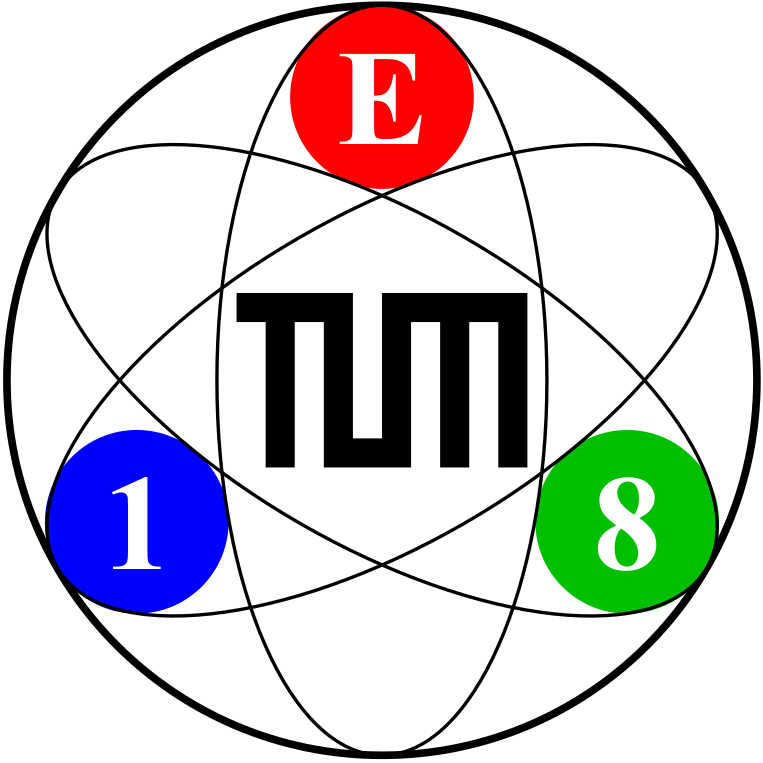
\includegraphics[width=0.8\textwidth]{E18Logo.png}
	\caption{Previous measurements of the proton radius}
	\label{fig:previous_proton_radius}
\end{figure}



\subsection{Elastic scattering of muons on protons}
The Amber experiment at CERN aims to reslove the proton radius puzzle, by measuring the elastic scattering of muons on protons as shown in figure \ref{fig:muon_proton_scatterin}.
\begin{figure}[h]
	\centering
	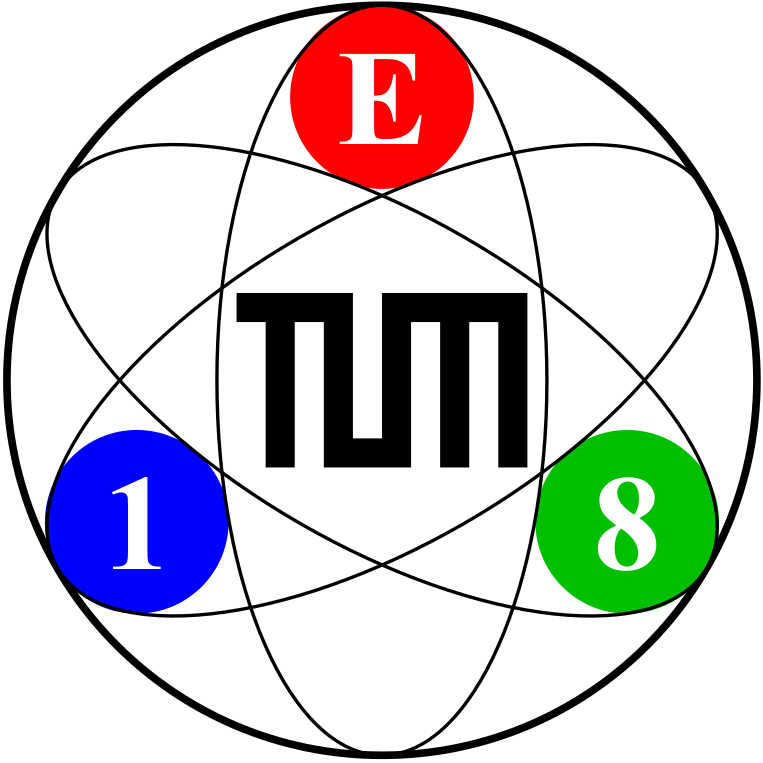
\includegraphics[width=0.8\textwidth]{E18Logo.png}
	\caption{Elastic scattering of muons with inc oming momentum p and outgoing momentum q on protons}
	\label{fig:muon_proton_scatterin}
\end{figure}

\newpage


\section{FPGA stuff}\label{sec:FPGAstuff}
here i will write about FPGAs and how they work and why they are used in the Amber experiment.
advantege of FPGAs is that they can be programmed to do a specific task, and that they are faster than CPUs for some tasks.